\documentclass[a4paper]{article}

\usepackage[utf8]{inputenc}
\usepackage{listings}
\usepackage{hyperref}
\usepackage{tikz}
\usepackage{scalefnt}
\usepackage{microtype}

\parindent 8pt
\parskip 2pt

\lstset{tabsize=2, basicstyle=\small, breaklines=true, numbers=left, language=c++}

\title{libea 0.2 - A short introduction}
\author{Sebastian Fedrau}
\date{November, 2014}

\begin{document}

\maketitle

\newpage

\section{Introduction}

\textsc{libea} is a template based library written in C++14. The purpose of this software is to provide an extensible and reliable framework for writing evolutionary algorithms.

\section{Building libea}

\textsc{libea} uses scons\footnote{\url{http://www.scons.org/}} as build system. To compile the library open the source code directory in a terminal and type in the following command:

\begin{lstlisting}[language=bash, numbers=none]
# scons libea
\end{lstlisting}

Now you can install the library:

\begin{lstlisting}[language=bash, numbers=none]
# scons install
\end{lstlisting}

After the installation the test suite can be build optionally. Please note that this step requires the CppUnit\footnote{\url{http://freedesktop.org/wiki/Software/cppunit/}} framework:

\begin{lstlisting}[language=bash, numbers=none]
# scons test-suite
\end{lstlisting}

I you want to build the source code documentation please ensure Doxygen\footnote{\url{http://www.stack.nl/~dimitri/doxygen/}} is installed on your system and type in the following command:

\begin{lstlisting}[language=bash, numbers=none]
# scons doc
\end{lstlisting}

\section{The framework}

\subsection{A quick overview}

In \textsc{libea} individuals are represented in \textit{sequences}. Theoretically any data type large enough to store the genotype of an individual could be used as sequence type. A group of sequences is called \textit{population}.

To modify a sequence or evaluate its fitness a corresponding \textit{genome base class} inherited from \textit{ea::AGenomeBase} is required. Figure~\ref{fig:overview} illustrates this concept.

\begin{figure}[h]
\caption{sequences and corresponding genome base class}
\label{fig:overview}
{\scalefont{0.6}
% Graphic for TeX using PGF
% Title: E:\git\libea\tex\img\overview.dia
% Creator: Dia v0.97.2
% CreationDate: Fri Nov 14 13:46:43 2014
% For: fedra001
% \usepackage{tikz}
% The following commands are not supported in PSTricks at present
% We define them conditionally, so when they are implemented,
% this pgf file will use them.
\ifx\du\undefined
  \newlength{\du}
\fi
\setlength{\du}{15\unitlength}
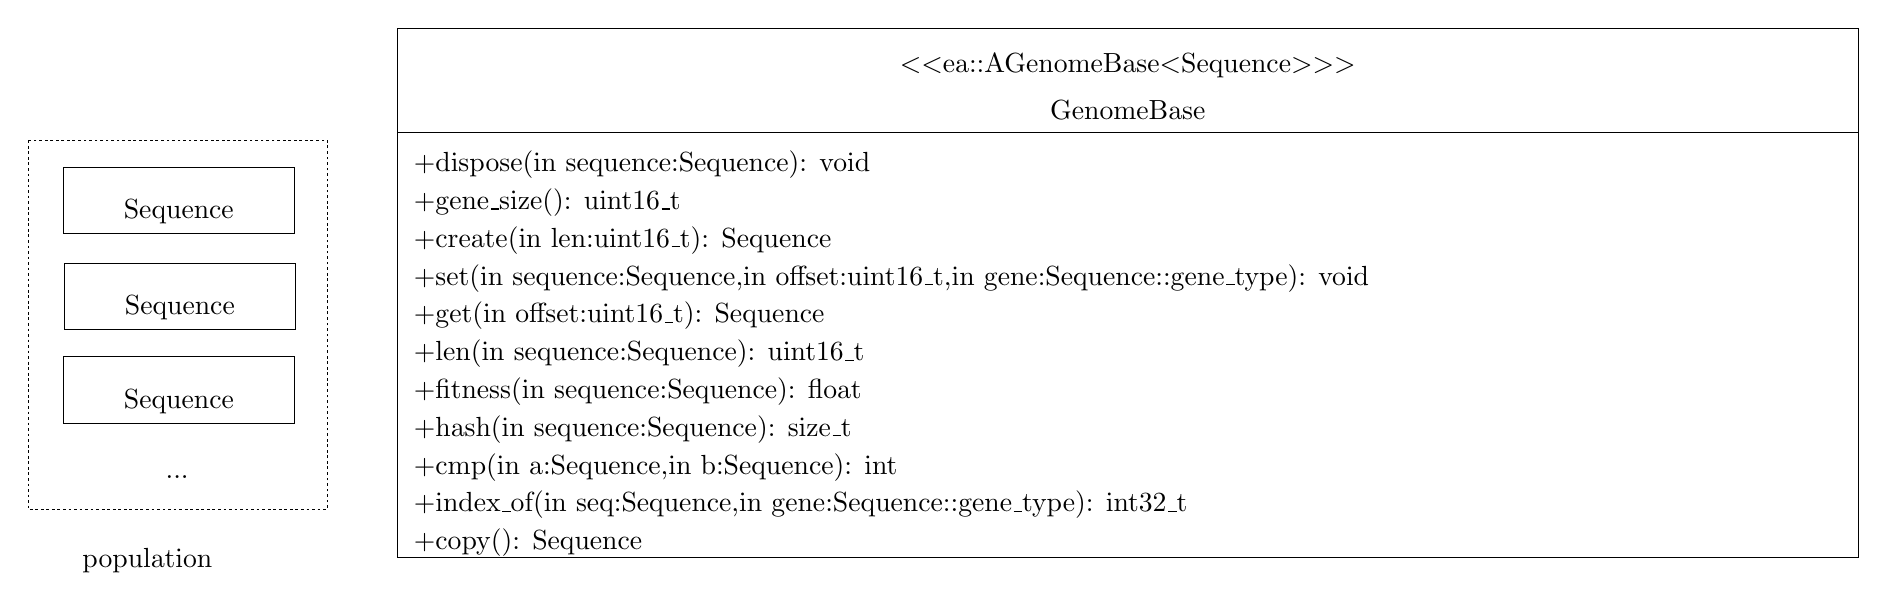
\begin{tikzpicture}[scale=0.6]
\pgftransformxscale{1.000000}
\pgftransformyscale{-1.000000}
\definecolor{dialinecolor}{rgb}{0.000000, 0.000000, 0.000000}
\pgfsetstrokecolor{dialinecolor}
\definecolor{dialinecolor}{rgb}{1.000000, 1.000000, 1.000000}
\pgfsetfillcolor{dialinecolor}
\pgfsetlinewidth{0.100000\du}
\pgfsetdash{{1.000000\du}{1.000000\du}}{0\du}
\pgfsetdash{{1.000000\du}{1.000000\du}}{0\du}
\pgfsetmiterjoin
\definecolor{dialinecolor}{rgb}{0.000000, 0.000000, 0.000000}
\pgfsetstrokecolor{dialinecolor}
\draw (18.942700\du,3.416490\du)--(18.942700\du,11.223911\du)--(25.285025\du,11.223911\du)--(25.285025\du,3.416490\du)--cycle;
\pgfsetlinewidth{0.100000\du}
\pgfsetdash{}{0pt}
\definecolor{dialinecolor}{rgb}{1.000000, 1.000000, 1.000000}
\pgfsetfillcolor{dialinecolor}
\fill (19.694000\du,3.977370\du)--(19.694000\du,5.377370\du)--(24.584000\du,5.377370\du)--(24.584000\du,3.977370\du)--cycle;
\definecolor{dialinecolor}{rgb}{0.000000, 0.000000, 0.000000}
\pgfsetstrokecolor{dialinecolor}
\draw (19.694000\du,3.977370\du)--(19.694000\du,5.377370\du)--(24.584000\du,5.377370\du)--(24.584000\du,3.977370\du)--cycle;
% setfont left to latex
\definecolor{dialinecolor}{rgb}{0.000000, 0.000000, 0.000000}
\pgfsetstrokecolor{dialinecolor}
\node at (22.139000\du,4.927370\du){Sequence};
\pgfsetlinewidth{0.100000\du}
\pgfsetdash{}{0pt}
\definecolor{dialinecolor}{rgb}{1.000000, 1.000000, 1.000000}
\pgfsetfillcolor{dialinecolor}
\fill (19.715600\du,6.007280\du)--(19.715600\du,7.407280\du)--(24.605600\du,7.407280\du)--(24.605600\du,6.007280\du)--cycle;
\definecolor{dialinecolor}{rgb}{0.000000, 0.000000, 0.000000}
\pgfsetstrokecolor{dialinecolor}
\draw (19.715600\du,6.007280\du)--(19.715600\du,7.407280\du)--(24.605600\du,7.407280\du)--(24.605600\du,6.007280\du)--cycle;
% setfont left to latex
\definecolor{dialinecolor}{rgb}{0.000000, 0.000000, 0.000000}
\pgfsetstrokecolor{dialinecolor}
\node at (22.160600\du,6.957280\du){Sequence};
\pgfsetlinewidth{0.100000\du}
\pgfsetdash{}{0pt}
\definecolor{dialinecolor}{rgb}{1.000000, 1.000000, 1.000000}
\pgfsetfillcolor{dialinecolor}
\fill (19.696300\du,7.992870\du)--(19.696300\du,9.392870\du)--(24.586300\du,9.392870\du)--(24.586300\du,7.992870\du)--cycle;
\definecolor{dialinecolor}{rgb}{0.000000, 0.000000, 0.000000}
\pgfsetstrokecolor{dialinecolor}
\draw (19.696300\du,7.992870\du)--(19.696300\du,9.392870\du)--(24.586300\du,9.392870\du)--(24.586300\du,7.992870\du)--cycle;
% setfont left to latex
\definecolor{dialinecolor}{rgb}{0.000000, 0.000000, 0.000000}
\pgfsetstrokecolor{dialinecolor}
\node at (22.141300\du,8.942870\du){Sequence};
% setfont left to latex
\definecolor{dialinecolor}{rgb}{0.000000, 0.000000, 0.000000}
\pgfsetstrokecolor{dialinecolor}
\node[anchor=west] at (21.660800\du,10.549200\du){...};
% setfont left to latex
\definecolor{dialinecolor}{rgb}{0.000000, 0.000000, 0.000000}
\pgfsetstrokecolor{dialinecolor}
\node[anchor=west] at (19.900600\du,12.303500\du){population};
\pgfsetlinewidth{0.100000\du}
\pgfsetdash{}{0pt}
\definecolor{dialinecolor}{rgb}{1.000000, 1.000000, 1.000000}
\pgfsetfillcolor{dialinecolor}
\fill (26.766600\du,1.034775\du)--(26.766600\du,3.234775\du)--(57.681600\du,3.234775\du)--(57.681600\du,1.034775\du)--cycle;
\definecolor{dialinecolor}{rgb}{0.000000, 0.000000, 0.000000}
\pgfsetstrokecolor{dialinecolor}
\draw (26.766600\du,1.034775\du)--(26.766600\du,3.234775\du)--(57.681600\du,3.234775\du)--(57.681600\du,1.034775\du)--cycle;
% setfont left to latex
\definecolor{dialinecolor}{rgb}{0.000000, 0.000000, 0.000000}
\pgfsetstrokecolor{dialinecolor}
\node at (42.224100\du,1.834775\du){\textless\textless ea::AGenomeBase\textless Sequence\textgreater\textgreater\textgreater};
% setfont left to latex
\definecolor{dialinecolor}{rgb}{0.000000, 0.000000, 0.000000}
\pgfsetstrokecolor{dialinecolor}
\node at (42.224100\du,2.784775\du){GenomeBase};
\definecolor{dialinecolor}{rgb}{1.000000, 1.000000, 1.000000}
\pgfsetfillcolor{dialinecolor}
\fill (26.766600\du,3.234775\du)--(26.766600\du,12.234775\du)--(57.681600\du,12.234775\du)--(57.681600\du,3.234775\du)--cycle;
\definecolor{dialinecolor}{rgb}{0.000000, 0.000000, 0.000000}
\pgfsetstrokecolor{dialinecolor}
\draw (26.766600\du,3.234775\du)--(26.766600\du,12.234775\du)--(57.681600\du,12.234775\du)--(57.681600\du,3.234775\du)--cycle;
% setfont left to latex
\definecolor{dialinecolor}{rgb}{0.000000, 0.000000, 0.000000}
\pgfsetstrokecolor{dialinecolor}
\node[anchor=west] at (26.916600\du,3.934775\du){+dispose(in sequence:Sequence): void};
% setfont left to latex
\definecolor{dialinecolor}{rgb}{0.000000, 0.000000, 0.000000}
\pgfsetstrokecolor{dialinecolor}
\node[anchor=west] at (26.916600\du,4.734775\du){+gene\_size(): uint16\_t};
% setfont left to latex
\definecolor{dialinecolor}{rgb}{0.000000, 0.000000, 0.000000}
\pgfsetstrokecolor{dialinecolor}
\node[anchor=west] at (26.916600\du,5.534775\du){+create(in len:uint16\_t): Sequence};
% setfont left to latex
\definecolor{dialinecolor}{rgb}{0.000000, 0.000000, 0.000000}
\pgfsetstrokecolor{dialinecolor}
\node[anchor=west] at (26.916600\du,6.334775\du){+set(in sequence:Sequence,in offset:uint16\_t,in gene:Sequence::gene\_type): void};
% setfont left to latex
\definecolor{dialinecolor}{rgb}{0.000000, 0.000000, 0.000000}
\pgfsetstrokecolor{dialinecolor}
\node[anchor=west] at (26.916600\du,7.134775\du){+get(in offset:uint16\_t): Sequence};
% setfont left to latex
\definecolor{dialinecolor}{rgb}{0.000000, 0.000000, 0.000000}
\pgfsetstrokecolor{dialinecolor}
\node[anchor=west] at (26.916600\du,7.934775\du){+len(in sequence:Sequence): uint16\_t};
% setfont left to latex
\definecolor{dialinecolor}{rgb}{0.000000, 0.000000, 0.000000}
\pgfsetstrokecolor{dialinecolor}
\node[anchor=west] at (26.916600\du,8.734775\du){+fitness(in sequence:Sequence): float};
% setfont left to latex
\definecolor{dialinecolor}{rgb}{0.000000, 0.000000, 0.000000}
\pgfsetstrokecolor{dialinecolor}
\node[anchor=west] at (26.916600\du,9.534775\du){+hash(in sequence:Sequence): size\_t};
% setfont left to latex
\definecolor{dialinecolor}{rgb}{0.000000, 0.000000, 0.000000}
\pgfsetstrokecolor{dialinecolor}
\node[anchor=west] at (26.916600\du,10.334775\du){+cmp(in a:Sequence,in b:Sequence): int};
% setfont left to latex
\definecolor{dialinecolor}{rgb}{0.000000, 0.000000, 0.000000}
\pgfsetstrokecolor{dialinecolor}
\node[anchor=west] at (26.916600\du,11.134775\du){+index\_of(in seq:Sequence,in gene:Sequence::gene\_type): int32\_t};
% setfont left to latex
\definecolor{dialinecolor}{rgb}{0.000000, 0.000000, 0.000000}
\pgfsetstrokecolor{dialinecolor}
\node[anchor=west] at (26.916600\du,11.934775\du){+copy(): Sequence};
\end{tikzpicture}

}
\end{figure}

\textsc{libea} offers the genome base class templates \textit{ea::PGenomeBase} and \textit{ea::CPGenomeBase} with the corresponding sequence types \textit{ea::Sequence} and \textit{ea::CSequence}. Any data type with a valid copy constructor is supported as gene type. There are already type aliases for many primitive data types available in \textsc{libea} (see table~\ref{tab:genome-base-classes-and-sequences}).

\begin{table}[h]
\begin{tabular}{|l|l|l|}
\hline
\textsc{genome base class} & \textsc{corresponding sequence type} & \textsc{gene type} \\
\hline
ea::PGenomeBase\textless T\textgreater & ea::Sequence\textless T\textgreater & T \\
ea::Int32PenomeBase & ea::Sequence\textless int32\_t\textgreater & int32\_t \\
ea::UInt32PGenomeBase & ea::Sequence\textless uint32\_t\textgreater & uint32\_t \\
ea::BinaryPGenomeBase & ea::Sequence\textless bool\textgreater & bool \\
ea::DoublePGenomeBase & ea::Sequence\textless double\textgreater & double \\
ea::StringPGenomeBase & ea::Sequence\textless std::string\textgreater & std::string \\
\hline
ea::CPGenomeBase\textless T\textgreater & ea::CSequence\textless T\textgreater & T \\
ea::Int32CPenomeBase & ea::CSequence\textless int32\_t\textgreater & int32\_t \\
ea::UInt32CPGenomeBase & ea::CSequence\textless uint32\_t\textgreater & uint32\_t \\
ea::BinaryCPGenomeBase & ea::CSequence\textless bool\textgreater & bool \\
ea::DoubleCPGenomeBase & ea::CSequence\textless double\textgreater & double \\
ea::StringCPGenomeBase & ea::CSequence\textless std::string\textgreater & std::string \\
\hline
\end{tabular}
\caption{genome base classes and corresponding sequence types offered by \textsc{libea}}
\label{tab:genome-base-classes-and-sequences}
\end{table}

The two offered templates are optimized for different use-cases. As shown in listing~\ref{lst:sequence} the \textit{ea::Sequence} structure has only two fields which are used to store the length of a sequence and its genes. Hence this kind of sequence is preferable if the application's memory footprint is critical.

In comparison the \textit{ea::CSequence} structure has three additional fields. They are used to cache evaluated fitness values and the hash of an individual (see listing~\ref{lst:csequence}). In general this sequence type is a better choice because the performance benefits might out weight the drawbacks of memory consumption.

The fields of both structures should \textbf{never be accessed directly}. \textsc{libea} provides the functions \textit{ea::sequence\_len()} and \textit{ea::sequence\_get()} for reading genes from a sequence.

\begin{lstlisting}[caption=Sequence template declaration, label=lst:sequence]
template<typename TGene>
struct Sequence
{
	/*! Datatype of stored genes. */
	typedef TGene gene_type;

	/*! Number of stored genes. */
	uint16_t len;
	/*! Dynamic array holding genes. */
	TGene* genes;
};
\end{lstlisting}

\begin{lstlisting}[caption=CSequence template declaration, label=lst:csequence]
template<typename TGene>
struct CSequence : Sequence<TGene>
{
	/*! Flags. */
	uint8_t flags;
	/*! Cached fitness value. */
	float fitness;
	/*! Cached hash value. */
	size_t hash;
};
\end{lstlisting}

\subsection{Core features}

\subsection{Working with sequences}

Listing~\ref{lst:core-functions} demonstrates some basic functions of \textsc{libea}. An individual represented in a sequence of integers is created (\textit{ll. 44-50}) and copied (\textit{l. 62}). The sequences are compared before and after modifying the second individual (\textit{ll. 67-75}).

To access the genes and evaluate the fitness a genome base class is declared (\textit{l. 22}). The template parameters specify gene type and fitness function (\textit{ll. 5-19}).

\begin{lstinputlisting}[caption=core functions,label=lst:core-functions]{examples/00-core-functions.cpp}
\end{lstinputlisting}

\subsection{Factories \& output adapters}

\textsc{libea} offers the \textit{ea::AFactory} base class as a unified way for creating populations. Listing~\ref{lst:factory} shows how to create sequences of ten random integers using a custom factory (\textit{ll. 30-51}). The values are generated with a random number generator (\textit{ll. 35-46}).

The individuals are written to an \textit{ea::OutputAdapter} (\textit{ll. 74-78}). At the current stage \textsc{libea} only provides an adapter for STL vectors, but new adapters can be added easily by implementing the \textit{ea::IOutputAdapter} interface.

\begin{lstinputlisting}[caption=custom factory,label=lst:factory]{examples/01-factory.cpp}
\end{lstinputlisting}

\subsection{Selection operators}

Selection operators have to implement the \textit{ea::IIndexSelection} interface (see listing~\ref{lst:iindexselection}). Instead of copying the selected genomes to an \textit{ea::OutpuAdapter} only the indexes are written. Access to the parent individuals is given through an adapter implementing the \textit{ea::IInputAdapter} interface. Input adapters can be created easily for all STL containers providing random access iterators with the \textit{ea::make\_input\_adapter()} function.

\begin{lstlisting}[caption=IIndexSelection,label=lst:iindexselection]
template<typename TGenomeBase>
class IIndexSelection
{
	public:
		typedef typename TGenomeBase::sequence_type sequence_type;

		~IIndexSelection() {}

		virtual void select(IInputAdapter<sequence_type>& input, const uint32_t count, IOutputAdapter<uint32_t>& output) = 0;
};
\end{lstlisting}

Listing~\ref{lst:selection-example} creates a population with ten random sequences  (\textit{ll. 43-58}). Then five individuals are selected using a tournament selection operator (\textit{ll. 72-83}).

\begin{lstinputlisting}[caption=selection operators,label=lst:selection-example]{examples/02-selection.cpp}
\end{lstinputlisting}

\subsection{Crossover operators}

Crossover operators are inherited from \textit{ea::ACrossover} and have to override the \textit{crossover()} method (see listing~\ref{lst:acrossover}). In the example two parent individuals are created (\textit{ll. 41-42}). Then two children are generated using a cycle crossover operator (\textit{ll. 51-56}). 

\begin{lstlisting}[caption=ACrossover,label=lst:acrossover]
template<typename TGenomeBase>
class ACrossover
{
	public:
		typedef typename TGenomeBase::sequence_type sequence_type;

		~ACrossover() {}

		virtual uint32_t crossover(const sequence_type& a, const sequence_type& b, IOutputAdapter<sequence_type>& output) = 0;
};
\end{lstlisting}

Crossover operators create at least one child sequence from two parent individuals. The \textit{crossover()} method returns the number of child sequences written to the given output adapter. Listing~\ref{lst:crossover-example} shows an example.

\begin{lstinputlisting}[caption=crossover operators,label=lst:crossover-example]{examples/03-crossover.cpp}
\end{lstinputlisting}

\subsection{Mutation operators}

Mutation operators are inherited from \textit{ea::AMutation} and have to override the \textit{create\_child()} method (see listing~\ref{lst:amutation}). 

\begin{lstlisting}[caption=AMutation,label=lst:amutation]
template<class TGenomeBase>
class AMutation
{
	public:
		typedef typename TGenomeBase::sequence_type sequence_type;

		virtual ~AMutation() {};

		virtual void mutate(sequence_type& sequence) = 0;

		sequence_type create_child(const sequence_type& sequence)
		{
			static TGenomeBase base;

			sequence_type m = base.copy(sequence);
			mutate(m);

			return m;
		}
};
\end{lstlisting}

In listing~\ref{lst:mutation-example} a parent individual is created (\textit{ll. 43-48}) and mutated in-place (\textit{l. 55}). Afterwards an inverted child sequence is generated (\textit{ll. 59-61}).

\begin{lstinputlisting}[caption=mutation operators,label=lst:mutation-example]{examples/04-mutation.cpp}
\end{lstinputlisting}

\section{Summary}

As you have seen in this tutorial \textsc{libea} provides a basic framework which may help you writing your own algorithms. There are some standard operators available which can be used with different kind of genomes, too.

The library has been written just for fun and I hope you might find it useful. To have a more detailed look at \textsc{libea} you should generate the code documentation as described before in this tutorial.
\end{document}